%% LyX 2.2.3 created this file.  For more info, see http://www.lyx.org/.
%% Do not edit unless you really know what you are doing.
\documentclass[oneside,reqno]{amsart}
\usepackage[T1]{fontenc}
\usepackage[utf8]{inputenc}
\pagestyle{plain}
\usepackage{mathrsfs}
\usepackage{amstext}
\usepackage{amsthm}
\usepackage{amssymb}
\usepackage{graphicx}
\usepackage{esint}
\usepackage[numbers]{natbib}
\usepackage[unicode=true,pdfusetitle,
 bookmarks=true,bookmarksnumbered=false,bookmarksopen=false,
 breaklinks=false,pdfborder={0 0 1},backref=section,colorlinks=false]
 {hyperref}

\makeatletter

%%%%%%%%%%%%%%%%%%%%%%%%%%%%%% LyX specific LaTeX commands.
%% Because html converters don't know tabularnewline
\providecommand{\tabularnewline}{\\}

%%%%%%%%%%%%%%%%%%%%%%%%%%%%%% Textclass specific LaTeX commands.
\numberwithin{equation}{section}
\numberwithin{figure}{section}

%%%%%%%%%%%%%%%%%%%%%%%%%%%%%% User specified LaTeX commands.
%2multibyte Version: 5.50.0.2960 CodePage: 1250


\usepackage{amsthm}
\usepackage{mathrsfs}
%\usepackage[notcite]{showkeys}
\usepackage{amsthm}
\usepackage{datetime}
\usepackage{mathrsfs}
\usepackage{amsthm}
\usepackage{amsfonts}
\usepackage{comment}
\setcounter{MaxMatrixCols}{30}
%TCIDATA{OutputFilter=latex2.dll}
%TCIDATA{Version=5.50.0.2960}
%TCIDATA{Codepage=1250}
%TCIDATA{CSTFile=amsart.cst}
%TCIDATA{Created=Wednesday, August 10, 2011 10:30:47}
%TCIDATA{LastRevised=Tuesday, November 03, 2015 14:08:24}
%TCIDATA{<META NAME="GraphicsSave" CONTENT="32">}
%TCIDATA{<META NAME="SaveForMode" CONTENT="1">}
%TCIDATA{BibliographyScheme=BibTeX}
%TCIDATA{<META NAME="DocumentShell" CONTENT="Articles\SW\bruce_plain">}
%TCIDATA{Language=American English}
%BeginMSIPreambleData
\providecommand{\U}[1]{\protect\rule{.1in}{.1in}}
%EndMSIPreambleData


\numberwithin{equation}{section}
\numberwithin{figure}{section}
\numberwithin{equation}{section}
\numberwithin{figure}{section}
\numberwithin{equation}{section}
\numberwithin{figure}{section}
\iffalse
\oddsidemargin= -0.2in
\evensidemargin= -0.2in
\textheight= 9in
\topmargin= -0.2in
\textwidth= 6.9in
\fi
\theoremstyle{plain}
\newtheorem{theorem}{Theorem}[section]
\newtheorem{corollary}[theorem]{Corollary}\newtheorem{lemma}[theorem]{Lemma}\newtheorem{convention}[theorem]{Convention}\newtheorem{mtheorem}[theorem]{Meta-Theorem}\newtheorem{proposition}[theorem]{Proposition}\newtheorem{htheorem}[theorem]{Heuristic Theorem}\newtheorem{axiom}{Axiom}\newtheorem{solution}[theorem]{Solution}\newtheorem{summary}[theorem]{Summary}\renewenvironment{proof}[1][Proof]{\textbf{#1.} }{\ \rule{0.5em}{0.5em}}
\theoremstyle{definition}
\newtheorem{definition}[theorem]{Definition}\newtheorem{comments}[theorem]{Comments}\newtheorem{notation}[theorem]{Notation}\newtheorem{notations}[theorem]{Notations}\newtheorem{example}[theorem]{Example}\theoremstyle{remark}
\newtheorem{remark}[theorem]{Remark}\newtheorem{remarks}[theorem]{Remarks}\newtheorem{fact}[theorem]{Fact}\theoremstyle{plain}
\newtheorem{conjecture}[]{Conjecture}\newtheorem{claim}[]{Claim}\newtheorem{computation}[]{Computation}\theoremstyle{definition}
\newtheorem{assumption}[]{Assumption}\newtheorem{exercise}{Exercise}[section]
\newtheorem{algorithms}[theorem]{Algorithm}\numberwithin{equation}{section}
\newcommand*{\bigchi}{\mbox{\Large$\chi$}}
\excludecomment{comments}

\makeatother

\begin{document}

\title{Training on Deep Neural Network (draft)}

\author{By Pun Wai Tong }

\date{10/03/17}

\email{punwai.tong@gmail.com}

\maketitle
\setcounter{section}{-1}

%\newpage

\section{Notations on Deep Neural Network}

All neural networks, e.g. convolution neural network and recurrent
neural network, share the same training spirit. In order to keep the
note simple and clear, let us consider training a fully connected
deep neural network for MNIST classification (supervised learning)
throughout the note.

\begin{definition} Let $d$ be a positive integer. Let $\{n_{i}\}_{i=1}^{d}\subseteq\mathbb{N}^{+}$
and $\{f_{i}\}_{i=2}^{d}$ is a set of activation functions, e.g.
$relu$, sigmoid and $tanh$. A $n$ -layer depth fully connected
deep neural network is a directed weighted graph (see Figure \ref{f.1.1})
such that 
\begin{enumerate}
\item the graph consists of $n$ layers (or called level) and the $i^{th}$
layer contains $n_{i}$ number of neurons (or called nodes) and an
activation function $f_{i}$(if $i\geq2$), 
\item two neurons are connected by an weighted edge only if the layer of
the neuron is next to that of the other neuro, 
\item the first layer is called input layer whose neuron values are fed
from the processed training data and the last layer is called the
output layer whose neuron values are compared with actual labels in
the training data. And all other layers are called hidden layers. 
\item By convention, $x_{j}^{i}$ stands for $j^{th}$ neuron value on the
$i^{th}$ layer and $w_{jk}^{i}$ corresponds to a weight from $j^{th}$
neuron on the $i^{th}$ layer to the $k^{th}$ neuron on the $(i+1)^{th}$
layer. Also, let $b_{j}^{i}$ is a biases value of a $j^{th}$neuron
on the $i^{th}$ layer. The relationship among neuron values are as
follows: for $d-2\geq i\geq1,$ the neuron value is 
\begin{equation}
x_{k}^{i+1}=f_{i+1}(\sum_{j=1}^{n_{i}}x_{j}^{i}w_{jk}^{i}+b_{k}^{i+1}).\label{e.1.1}
\end{equation}
for $i=d-1,$ 
\begin{equation}
\left\{ x_{k}^{d}\right\} _{k=1}^{n_{d}}=f_{d}\left(\left\{ \sum_{j=1}^{n_{d-1}}x_{j}^{d-1}w_{jk}^{d-1}+b_{k}^{d}\right\} _{k=1}^{n_{d}}\right)\label{e.1.2}
\end{equation}
\end{enumerate}
\end{definition}

\begin{figure}
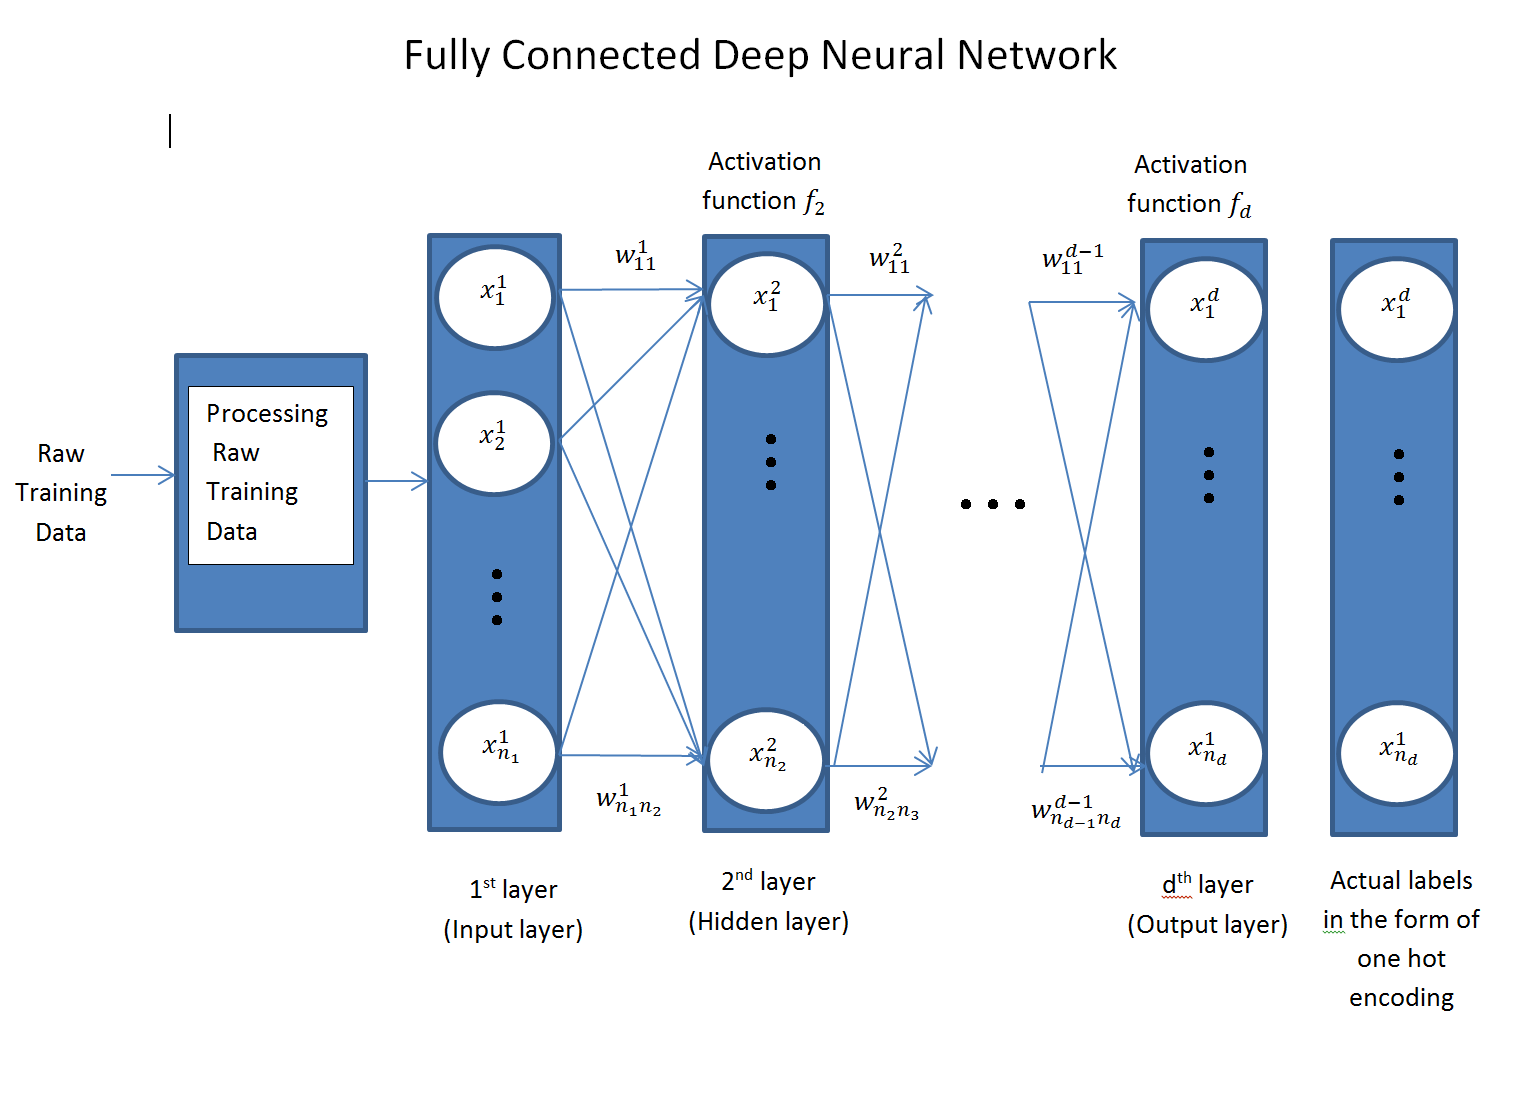
\includegraphics[scale=0.3]{FCDNN}

\protect\caption{A $d$-layer depth fully connected deep neural network\label{f.1.1}}
\end{figure}

\section{Processing Training Data}

In order to boost up the accuarcy performance of the neural network,
raw training data are processed before being fed to the neural network.
There are many ways to process raw training data depending on many
factors, e.g. the nature of training data itself and the type of deep
neural network. For example, raw data of MNIST data set are images
which are represented by an array of pixels value (may transform from
a matrix to an array if necessary) ranging from $0$ to 255. If the
first two layer of the deep neural network corresponding to restricted
Boltzmann machine to learn features, then the raw data of MNIST data
set is transformed to a binary values which is either $0$ or $1.$
In our example of MNIST classification using a fully connected deep
neural network, each pixel value $x$ of an image in MNIST data set
is proceeded by a transformation $T$ 
\[
T\left(x\right)=\frac{x-\frac{255}{2}}{\frac{255}{2}}.
\]
so that the value of each input data is symmetric about $0$ and lies
in $\left[-1,1\right]$.

\begin{remark} In our example of MNIST classification using a fully
connected deep neural network, the size of an image is $28\times28$
pixels. The number of neurons in the $1^{st}$ layer (input layer),
$n_{1}$ , is $28\times28$.\end{remark}

\section{Representation of LAbels in supervised training}

In the supervised training, each training example corresponds to a
label. For example, in the MNIST data set, a training example is an
image while the corresponding label is a digit shown in the image
. The label is transformed to a representation so that conclusion,
e.g. similarity can be drawn by comparing between the representation
and the neuron values in the output layer. One common representation
of the MNIST data set is one hot encoding. Suppose MNIST data set
contains images of digits from $1$ to $10$. In the form of one hot
encoding, the $k^{th}$ digit is represented by a column vector with
$10$ entries such that the only $k^{th}$ entry is $1$ and all other
entries are $0$ (see Figure \ref{f.3.1}). 
\begin{figure}
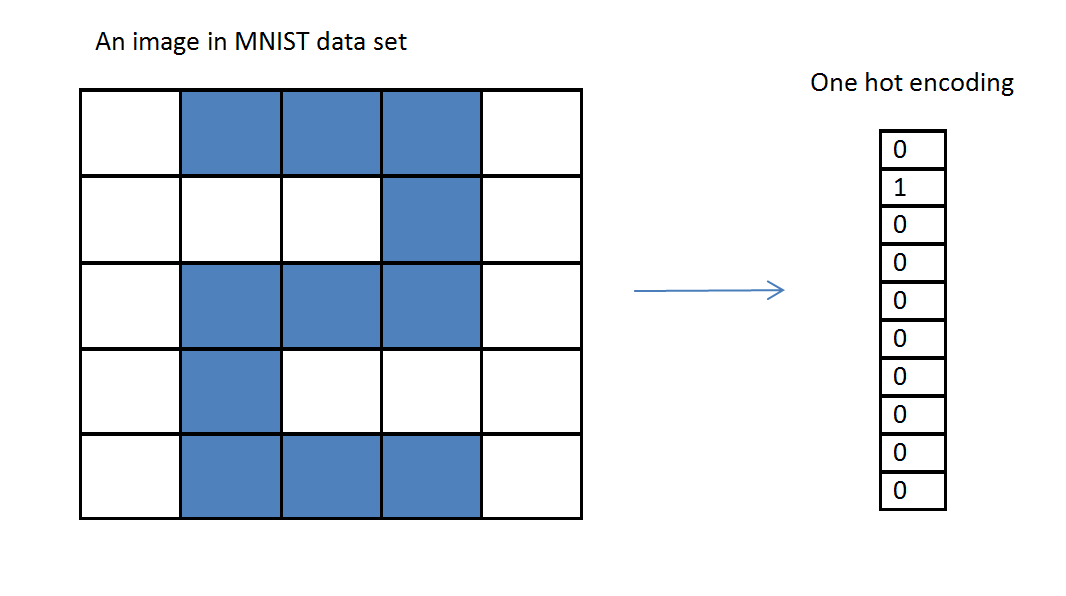
\includegraphics[scale=0.3]{MNIST_Example}

\protect\caption{Training Example and Label of MNIST. The training example is the image
of digit $2$ and the label is $2$. The column matrix on the right
is the representation of a digit 2 by using one hot encoding. \label{f.3.1}}
\end{figure}

\begin{remark} Since MNIST data set is assumed to contain images
of digits from $1$ to $10$. The number of neurons in the $d^{st}$
layer (output layer), $n_{d}$ , is $10$.\end{remark}

\section{Activation Function\label{s.4}}

Choices of activation functions $f(x)$ are keys to train a deep neural
network successfully. Inapropriate activations function could make
the deep neural network difficult to be trained. There are some requirements
of activation functions. For example, 
\begin{enumerate}
\item the activation function $f(x)$ is easy to compute. 
\item the activation function $f(x)$ cannot grow too fast as $\left|x\right|$
grows otherwise overflow may occur for neuron values, especially if
the neuron network is very huge (i.e., large number of neurons in
each layer) and deep (i.e., many layers). 
\item the activation function $f(x)$ is differentiable and its derivatives
is easy to compute. 
\item the derivative of activation function should not vanish when $\left|x\right|$grows,
i.e. $|f^{'}(x)|\rightarrow0$ as $\left|x\right|\rightarrow\infty.$
An activation function having this property is called a non-saturated
function. 
\end{enumerate}
In our example of MNIST classification, activation functions $f_{k}^{i}$
from the $2^{nd}$ layer to the $(d-1)^{th}$ layer (for $2\leq i\leq d-1$
and $1\leq k\leq n_{i}$) are $Relu$ function which is defined as
\[
Relu(x):=\begin{cases}
x & \textrm{if }x\geq0\\
0 & \textrm{otherwise}
\end{cases}.
\]

It can be seen that 
\[
\left(Relu\right)^{'}(x)=\begin{cases}
1 & \textrm{if }x>0\\
0 & x<0
\end{cases}.
\]
The activation function $Relu$ is differentiable everywhere except
$x=0$ and its derivative is easy to compute. Also, $Relu$ is non-saturated.
Therefore, $Relu$ satisfies the $1^{st}$, $3^{nd}$ and $4^{th}$
requirement of the activation function mentioned above. Owing to the
unclear description of the $2^{nd}$ requirement of the activation
function, it is hard to justify if $Relu$ satisfies the requirement.
But practical experience shows that overflow of neuron values are
rarely caused by $Relu$ function. All these reason makes $Relu$
one of the most popular activation functions nowaday.

The activation function $f_{d}\left(\cdot\right)$ in the output layer
isvery special and different from all activation functions in other
layers. First, the $1^{st}$, $2^{nd}$ and $4^{th}$ activation function
requirement are not valued too much for $f_{d}$. But the range of
the activation function $f_{d}(\cdot)$ is required to be between
$0$ and $1$ such that $\sum_{k=1}^{n_{d}}x_{k}^{n}=1$ (normalization
requirement). The reason for the normalization requirement is to view
the value of the $j^{th}$ neuron on the output layer as the probability
of the training example belonging to the $j^{th}$ class.By convention,
let us define the notations of neuron value before activation.

\begin{notation} \label{n.4.1}Let $\tilde{x}_{k}^{i+1}$ is the
$k^{th}$ neuron value on the $i+1^{th}$ layer before activation,
i.e. for $d-1\geq i\geq1$ 
\begin{equation}
\tilde{x}_{k}^{i+1}=\sum_{j=1}^{n_{i}}x_{j}^{i}w_{jk}^{i}+b_{k}^{i+1}.\label{e.4.1}
\end{equation}

and 
\begin{equation}
x_{k}^{i+1}=f^{i+1}\left(\tilde{x}_{k}^{i+1}\right)\label{e.4.2}
\end{equation}
where $f^{i+1}$ be an activation function on the $\left(i+1\right)^{th}$
layer. \end{notation}

In order to achieve the normalization requirement, $f_{d}\left(\cdot\right)$
rely on all neurons value before activation in the output layer, i.e.$f_{d}:\mathbb{R}^{n_{d}}\rightarrow[0,1]^{n_{d}}$
(c.f. $Relu:\mathbb{R\rightarrow\mathbb{R}})$. In our example of
MNIST classification, the activation function in the output layer,
$f_{d}$, is a $softmax$ function defined as

\begin{eqnarray*}
softmax:\mathbb{R}^{n_{d}} & \rightarrow & [0,1]^{n_{d}}
\end{eqnarray*}
\[
\left(y_{1},...,y_{n_{d}}\right)=\left(\frac{\exp(y_{1})}{\sum_{j=1}^{n_{d-1}}\exp(y_{j})},...,\frac{\exp(y_{n_{d}})}{\sum_{j=1}^{n_{d-1}}\exp(y_{j})}\right).
\]

Note that $n_{d}=10$ in our example and the $k^{th}$ neuron value
which is $x_{k}^{d}=j^{th}\textrm{ component of }$$softmax\left(\left\{ \tilde{x}_{j}^{d}\right\} _{j=1}^{n_{d}}\right)$
is interpreted as the probability of the training example belonging
to $j^{th}$ digit.

\begin{remark} A function is called saturated if the function is
not non-saturated. A saturated function brings troubles to train a
neural network because it is hard to learn. {[}Say it in training
or appendix{]}. \end{remark}

\section{Loss function}

Loss function is another important criteria for successful training
of a deep neural network. Given a set of training examples, the loss
function is a real-valued function of parameters (weights and biases
in a deep neural network).The construction of a loss function depends
on the task and the structure of a deep neural network model. For
example, the loss function of the restricted Boltzmann machine for
unsupervised learning is about the probability occurrence of some
training examples. In our example of classification on MNIST data
set by fully connected deep neural network, the loss function is about
the error difference between predicted digits and actual digits for
some training examples. Before formulating a loss model, let us introduce
some notations first.

\begin{notation} \label{n.5.1} Let $T$ be a mini-batch which is
a subset of the training data and 
\begin{equation}
\theta=\left\{ w_{jk}^{i},b_{k}^{i+1}\textrm{ }|\textrm{ }0\leq i\leq d-1\textrm{ and }1\leq j\leq n_{i}\textrm{ and }1\leq k\leq n_{i+1}\}\right\} \label{e.5.1}
\end{equation}
be a set of training parameters. Given $t\in T,$ we notate $x_{j}^{i}(t)$
as the $j^{th}$ neuron value on the $i^{th}$ layer by inputting
training example $t$ to the fully connected deep neural network.
We also notate $\{y_{j}(t)\}_{j=1}^{n_{d}}$ to be the one hot encoding
representation of the $j^{th}$ label (it is a digit in our example).
\end{notation}

IIn our example of MNIST classification, a cross entropy is used to
measure the difference between the predicted label and actual label.

\begin{definition}The loss function $L$ in our example is defined
as 
\begin{equation}
L(\theta|T)=\frac{1}{\left|T\right|}\sum_{t\in T}\sum_{k=1}^{n_{d}}y_{k}(t)log\left(x_{k}^{d}(t)\right).\label{e.5.2}
\end{equation}

Just a reminder that $x_{i}^{d}$ does not mean $x_{i}$ to the power
$d$ but the $k^{th}$ neuron value in the $d^{th}$ layer. Note that
there is only one non-zero term in the inner summation in Eq. (\ref{e.5.2}).
\end{definition}

\section{\label{s.6} Initialization of training parameters}

Values of training parameters which are weights and biases are initialized
in a deep neural network. Owing to being huge and deep in the neural
network model, an inappriporiate initialization leads to many problems
in the training, e.g. overflow in the neuron values occurs and neuron
values lie in the saturated region (see the Appendix). At the end
of the day, the neural network cannot learn from training data. Some
schemes are introduced for the initialization of training parameters.
One common scheme is Xavier initialization which are designed to apply
the deep neural network if activation functions on all but the last
layer are $tanh$ or sigmoid.

\begin{definition} \label{d.6.1} Let $\mu\in\mathbb{R}$ and $\sigma>0$
and $N\left(\mu,\sigma\right)$ be a Gaussian distribution with mean
$\mu$ and standard deviation $\sigma.$ Xavier Initiailization initializes
weights and biases in the following way for $0\leq i\leq d-1.$ 
\begin{enumerate}
\item If the activation function is $tanh$ and sigmoid, weights $w_{jk}^{i}$
are initialized by a random number drawn from $N(0,\frac{1}{\sqrt{n_{i}+n_{i+1}}}).$ 
\item Biases $b_{k}^{i+1}$ is initialized to be zero. 
\end{enumerate}
\end{definition}

Another common initialization scheme for $Relu$ activation function
is studied by \citep{Zhang2015} written by K. He, X, Zhang, S. Ren
and J. Sun. We will use the scheme in our MNIST classification example
and the scheme is defined as follows:

\begin{definition} \label{d.6.2} He, Zhan, Ren and Sun's initialization
scheme initializes weights and biases in the following way for $0\leq i\leq d-1.$ 
\begin{enumerate}
\item If the activation function is $Relu$ on all but the last layer, weights
$w_{jk}^{i}$ are initialized by a random number drawn from $N(0,\frac{2}{\sqrt{n_{i}}}).$ 
\item Biases $b_{k}^{i+1}$ is initialized to be zero. 
\end{enumerate}
\end{definition}

Loosely speaking, a main spirit of both schemes is to keep the variance
of neuron values before activation in all layers almost the same.
To illustrate the spirit, let us show the argument in He, Zhan, Ren
and Sun's initialization scheme.

\begin{theorem} Assume $x_{j}^{0}$ from Notation \ref{n.4.1} follows
the same symmetric probability density distribution (aka pdf) around
$0$ for $0\leq i\leq d-2$ and $0\leq j\leq n_{i}$. Suppose weights
$w_{jk}^{i}$ and neuron values $x_{j}^{0}$ are all independent random
variables. If 
\begin{equation}
var\left[w_{jk}^{i}\right]=\frac{2}{n_{i}}\label{e.6.1}
\end{equation}
hold, then, under He, Zhan, Ren and Sun's initialization scheme, there
exists a constant $c\geq0$ such that the neuron relationship from
Eq.(\ref{e.1.1}) leads to 
\begin{equation}
Var\left[\tilde{x}_{j}^{i}\right]=c.\label{e.6.2}
\end{equation}

for $1\leq i\leq d-1$ and $1\leq j\leq n_{i}$.

\end{theorem}

\begin{proof} From Eq.(\ref{e.1.1}), $\tilde{x}_{k}^{1}$ is a sum
of a product of independent weights $w_{jk}^{0}$ and neuron values
$x_{j}^{0}$ which are assumed to be independent and follow a symmetric
pdf around $0.$ Therefore, $\tilde{x}_{k}^{1}$ follows the symmetric
pdf around $0$ and same the same variance among all $k$. Therefore,
using Eq.(\ref{e.1.1}) where $i=1$, we learn $\tilde{x}_{k}^{2}$
share the same symmetric pdf near $0$ and 
\begin{eqnarray}
Var\left[\tilde{x}_{k}^{2}\right] & = & \sum_{j=1}^{n_{1}}Var\left(x_{j}^{1}w_{jk}^{1}\right)=\sum_{j=1}^{n_{1}}Var\left(w_{jk}^{1}\right)E\left[\left(x_{j}^{1}\right)^{2}\right]\nonumber \\
 & = & n_{1}Var\left[w_{11}^{1}\right]E\left[\left(x_{1}^{1}\right)^{2}\right].\label{e.6.3}
\end{eqnarray}

By using Eq. (\ref{e.6.1}), we can conclude that and an update function
$g:\mathbb{R}\times\mathbb{R}\times S\rightarrow\mathbb{R}$ where
$S$ could be an empty space. 
\begin{equation}
Var\left[\tilde{x}_{k}^{2}\right]=E\left[\left(x_{1}^{1}\right)^{2}\right].\label{e.6.4}
\end{equation}

Let $dp$ be a probability measure for $\tilde{x}_{1}^{1}$. Since
$x_{1}^{1}=Relu\left(\tilde{x}_{1}^{1}\right)$, we have 
\begin{equation}
E\left[\left(x_{1}^{1}\right)^{2}\right]=\int_{\tilde{x}_{k}^{1}>0}\left(\tilde{x}_{1}^{1}\right)^{2}dp=\frac{1}{2}\int_{\mathbb{R}}\left(\tilde{x}_{1}^{1}\right)^{2}dp=\frac{1}{2}E\left[\left(\tilde{x}_{1}^{1}\right)^{2}\right].\label{e.6.5}
\end{equation}

The second equality of Eq. (\ref{e.6.5}) is because of $\tilde{x}_{1}^{1}$
having the symmetric pdf around $0.$ Since $\tilde{x}_{k}^{1}$ has
the mean zero, we have 
\begin{equation}
E\left[\left(\tilde{x}_{k}^{1}\right)^{2}\right]=Var\left[\tilde{x}_{1}^{1}\right].\label{e.6.6}
\end{equation}

Combining all Eqs (\ref{e.6.3}), (\ref{e.6.4}), (\ref{e.6.5}) and
(\ref{e.6.6}), we can conclude that for all $1\leq k\leq n_{2}$
\[
Var\left[\tilde{x}_{k}^{2}\right]=Var\left[\tilde{x}_{1}^{1}\right].
\]

By induction, Eq. (\ref{e.6.6}) is asserted.

\end{proof}

\section{Training in Deep neural Netowrk}

In order to compute update all weights $w_{jk}^{i}$ and biases $b_{k}^{i+1}$
of the loss function $L$ in Eq. (\ref{e.5.2}) efficiently in terms
of speed and memory, there are two steps in the training of deep neural
network: forward propagation and back propagation.

\subsection{Forward Propagation}

Let $T$ be a mini-batch. Suppose values of 
\[
\left\{ w_{jk}^{i}\right\} _{1\leq j\leq n_{i},1\leq k\leq n_{i+1},1\leq i\leq d-1}\textrm{ and }\left\{ b_{j}^{i}\right\} _{1\leq j\leq n_{i},2\leq i\leq d}
\]
are given. Forward propgation is to compute the neuron values of $x_{k}^{i}(t)$
layer by layer from left to right in Figure \ref{f.1.1} through Eqs.
(\ref{e.1.1}) and (\ref{e.1.2}) for each $t\in T,$ . For example,
we first compute $\left\{ x_{k}^{2}(t)\right\} _{k=1}^{n_{2}}$ in
the $2^{nd}$ layer by pluging neuron value $\left\{ x_{j}^{1}(t)\right\} _{j=1}^{n_{1}}$
in the first layer (input layer) through Eq. (\ref{e.1.1}). Therefore,
values of neurons in all layers are known after forward propgation.
The implementation of forward propagation is summarized in the following
algorithm.

\begin{algorithms} \label{a.7.1} Forward Propagation: 
\begin{itemize}
\item Inputs: a mini batch set $T$ , $\left\{ w_{jk}^{i}\right\} _{1\leq j\leq n_{i},1\leq k\leq n_{i+1},1\leq i\leq d-1}$
and $\left\{ b_{k}^{i+1}\right\} _{1\leq k\leq n_{i+1},1\leq i\leq d-1}$ 
\item Outputs: $\left\{ x_{j}^{i}(t)\right\} _{1\leq j\leq n_{i},1\leq i\leq d,t\in T}$ 
\item Algorithm: 
\begin{enumerate}
\item Set $i=2$ 
\item If $i=d$, then compute $x_{j}^{i}\left(t\right)$ by Eq. (\ref{e.1.2})
for all $1\leq j\leq n_{i}$ and for $t\in T$. Otherwise, compute
$x_{j}^{i}\left(t\right)$ by Eq. (\ref{e.1.1}) for all $1\leq j\leq n_{i}$
and for $t\in T$. 
\item Update $i$ by $i+1$ 
\item Go to Step $2$ until $i=d$ 
\end{enumerate}
\end{itemize}
\end{algorithms}

\subsection{Back Propagation}

Given all neuron values, back progation is to compute the derivatives
of the loss function $L$ in Eq. (\ref{e.5.2}) with respect to each
weight $w_{jk}^{i}$ and biases $b_{k}^{i+1}$ layer by layer from
right to left in Figure \ref{f.1.1} to update 
\[
\textrm{weight }\left\{ w_{jk}^{i}\right\} _{1\leq j\leq n_{i},1\leq k\leq n_{i+1},1\leq i\leq d-1}\textrm{ and }\textrm{biases }\left\{ b_{j}^{i}\right\} _{1\leq j\leq n_{i},2\leq i\leq d}
\]
How the back propgation is implemented? Let us start a new notation
for illustration of back propagation.

\begin{definition} \label{d.7.1} Let $\tilde{x}_{j}^{i}$ be as
in Notation (\ref{n.4.1}) and $L$ be a loss function in Eq. (\ref{e.5.2}).
Let $T$ be a mini-batch. For $t\in T,$ an error derivative 
\begin{equation}
E_{j}^{i}(t):=\frac{\partial L}{\partial\tilde{x}_{j}^{i}}\left(\theta|\{t\}\right)\label{e.7.1}
\end{equation}
is defined as a derivative of $L$ with respect to $\tilde{x}_{j}^{i}$
evaluated at $\tilde{x}_{j}^{i}(t)$ for $2\leq i\leq d$ and $1\leq j\leq n_{i}.$
\end{definition}

The main idea of the back propgation is to derive a recursive relationship
between $\left\{ E_{j}^{i}\left(t\right)\right\} _{j=1}^{n_{i}}$
and $\left\{ E_{k}^{i+1}\left(t\right)\right\} _{k=1}^{n_{i+1}}$
by using a chain rule and compute $\frac{\partial L\left(\theta|T\right)}{\partial w_{jk}^{i}}$
and $\frac{\partial L\left(\theta|T\right)}{\partial b_{k}^{i+1}}$
based on $\left\{ E_{k}^{i+1}\left(t\right)\right\} _{k=1,t\in T}^{n_{i+1}}$.

First, let us derive the recursive relationship between $\left\{ E_{j}^{i}\left(t\right)\right\} _{j=1}^{n_{i}}$
and $\left\{ E_{k}^{i+1}\left(t\right)\right\} _{k=1}^{n_{i+1}}$
in the following lemma.

\begin{lemma} \label{l.7.1}All notations are as above. For $2\leq i\leq d-1$,
$1\leq j\leq n_{i}$ and $1\leq k\leq n_{i+1}$, we have 
\begin{equation}
E_{j}^{i}(t)=\sum_{k=1}^{n_{i+1}}E_{k}^{i+1}(t)w_{jk}^{i}(f^{i})^{'}|_{\tilde{x}_{j}^{i}(t)}\label{e.7.2}
\end{equation}
where $(f^{i})^{'}|_{\tilde{x}_{j}^{i}(t)}$ is the derivative of
an activation function $f^{i}$(see Section \ref{s.4}) on the $i^{th}$
layer evaluated at $\tilde{x}_{j}^{i}(t).$ {[}Note $L\left(\theta|\{t\}\right)=y_{i}(t)log\left(x_{i}^{d}(t)\right)$
from Eq. (\ref{e.5.2}) {]} \end{lemma}

\begin{proof} The proof is by a direct computation. 
\begin{eqnarray*}
E_{j}^{i}(t) & = & \frac{\partial L}{\partial\tilde{x}_{j}^{i}}\left(\theta|\left\{ t\right\} \right)=\frac{\partial L}{\partial\tilde{x}_{j}^{i}}|_{\tilde{x}_{j}^{i}(t)}\\
 & = & \sum_{k=1}^{n_{i+1}}\frac{\partial L}{\partial\tilde{x}_{k}^{i+1}}|_{\tilde{x}_{k}^{i+1}(t)}\frac{\partial\tilde{x}_{k}^{i+1}}{\partial x_{j}^{i}}|_{x_{j}^{i}(t)}\frac{\partial x_{j}^{i}}{\partial\tilde{x}_{j}^{i}}|_{\tilde{x}_{j}^{i}(t)}\\
 & = & \sum_{k=1}^{n_{i+1}}E_{k}^{i+1}w_{jk}^{i}(f^{i})^{'}|_{\tilde{x}_{j}^{i}(t)}.
\end{eqnarray*}

The last equality is because of Eqs. (\ref{e.4.1}), (\ref{e.4.2})
and (\ref{e.7.1}).\end{proof}

The following lemma illustrates how to compute $\frac{\partial L}{\partial w_{jk}^{i}}$
and $\frac{\partial L}{\partial b_{k}^{i+1}}$ by using $\left\{ E_{k}^{i+1}\right\} _{k=1}^{n_{i+1}}$.

\begin{definition} \label{d.7.2}Let $k,\ell\in\mathbb{N}.$ Then,
a kronecker delta $\delta_{k,\ell}$ is defined as 
\[
\delta_{k,\ell}:=\begin{cases}
1 & \textrm{if }k=\ell\\
0 & \textrm{otherwise}
\end{cases}
\]

\end{definition}

\begin{lemma} \label{l.7.2}All notations are as above. Given the
mini batch set $T$, for $1\leq i\leq d-1$, $1\leq j\leq n_{i}$
and $1\leq k\leq n_{i+1}$, the derivative of the loss function $L\left(\theta|T\right)$
with respect to its trainining parameters $\theta$becomes 
\begin{equation}
\frac{\partial L}{\partial w_{jk}^{i}}(\theta|T)=\sum_{t\in T}E_{k}^{i+1}(t)x_{j}^{i}(t)\textrm{ and }\frac{\partial L}{\partial b_{k}^{i+1}}(\theta|T)=\sum_{t\in T}E_{k}^{i+1}(t).\label{e.7.3}
\end{equation}
\end{lemma}

\begin{proof} From Eq. (\ref{e.5.2}), we can learn that 
\[
L\left(\theta|\{t\}\right)=y_{i}(t)log\left(x_{i}^{d}(t)\right)\textrm{ and }L\left(\theta|T\right)=\frac{1}{T}\sum_{t\in T}L\left(\theta|\{t\}\right).
\]

By linearity of differentiation, it suffice for us to show 
\begin{equation}
\frac{\partial L}{\partial w_{jk}^{i}}(\theta|\left\{ t\right\} )=E_{k}^{i+1}(t)x_{j}^{i}(t)\textrm{ and }\frac{\partial L}{\partial b_{k}^{i+1}}(\theta|\left\{ t\right\} )=E_{k}^{i+1}(t).\label{e.7.4}
\end{equation}

By using a chain rule and Eq. (\ref{e.4.1}), Eq.(\ref{e.7.4}) becomes
\begin{eqnarray*}
\frac{\partial L}{\partial w_{jk}^{i}}\left(\theta|\{t\}\right) & = & \sum_{\ell=1}^{n_{i+1}}\frac{\partial L}{\partial\tilde{x}_{\ell}^{i+1}}\frac{\partial\tilde{x}_{\ell}^{i+1}}{\partial w_{jk}^{i}}=\sum_{\ell=1}^{n_{i+1}}E_{\ell}^{i+1}x_{j}^{i}\delta_{\ell,k}=E_{k}^{i+1}(t)x_{j}^{i}(t)
\end{eqnarray*}
and 
\[
=\frac{\partial L}{\partial b_{k}^{i+1}}(\theta|\left\{ t\right\} )=\sum_{\ell=1}^{n_{i+1}}\frac{\partial L}{\partial\tilde{x}_{\ell}^{i+1}}\frac{\partial\tilde{x}_{\ell}^{i+1}}{\partial w_{jk}^{i}}=\sum_{\ell=1}^{n_{i+1}}E_{\ell}^{i+1}\delta_{\ell,k}=E_{k}^{i+1}(t).
\]

The lemma follows.

\end{proof}

From Lemma \ref{l.7.1} and \ref{l.7.2}, the back propagation is
implemented as follows.

\begin{definition} \label{d.7.3} An update scheme $G$ is a scheme
to update weights $\left\{ w_{jk}^{i}\right\} _{1\leq j\leq n_{i},1\leq k\leq n_{i+1},1\leq i\leq d-1}$
and biases $\left\{ b_{k}^{i+1}\right\} _{1\leq k\leq n_{i+1},1\leq i\leq d-1}$
in a deep neural network by using current weights and derivatives
as inputs (they may not be the only inputs in the scheme). \end{definition}

\begin{algorithms} \label{a.7.2} Back Propagation Algorithm: 
\begin{itemize}
\item Inputs: $\left\{ w_{jk}^{i}\right\} _{1\leq j\leq n_{i},1\leq k\leq n_{i+1},1\leq i\leq d-1}$,
$\left\{ b_{k}^{i+1}\right\} _{1\leq k\leq n_{i+1},1\leq i\leq d-1}$
, neuron values $\left\{ x_{j}^{i}(t)\right\} _{1\leq j\leq n_{i},1\leq i\leq d,t\in T}$,
actual labels of training data $T$ $\left\{ y_{i}(t)\right\} _{1\leq i\leq n_{d},t\in T}$
and an update scheme $G$ in Definition \ref{d.7.3}. 
\item Outputs: $\left\{ w_{jk}^{i}\right\} _{1\leq j\leq n_{i},1\leq k\leq n_{i+1},1\leq i\leq d-1}$
and $\left\{ b_{k}^{i+1}\right\} _{1\leq k\leq n_{i+1},1\leq i\leq d-1}$ 
\item Algorithm: 
\begin{enumerate}
\item Set $i=d-1$ 
\item If $i=d-1,$ compute $E_{k}^{i+1}(t)$ for $1\leq k\leq n_{i-1}$
by Eq. (\ref{e.7.1}). Otherwise, compute $E_{k}^{i+1}(t)$ for $1\leq k\leq n_{i-1}$
by Eq. (\ref{e.7.2}). 
\item Compute $\frac{\partial L}{\partial w_{jk}^{i}}(\theta|T)$ and $\frac{\partial L}{\partial b_{k}^{i+1}}(\theta|T)$
for $1\leq j\leq n_{i}$ and $1\leq k\leq n_{i+1}$ by using \ref{e.7.3}
where $T$ is $\left\{ x_{j}^{1}(t)\right\} _{1\leq j\leq n_{1},t\in T}$ 
\item For $1\leq j\leq n_{i}$ and $1\leq k\leq n_{i+1},$ update weights
$w_{jk}^{i}$ and biases $b_{k}^{i+1}$ by using the update scheme
$G$ with inputs $\left\{ y_{i}(t)\right\} _{1\leq i\leq n_{d},t\in T}$,
$w_{jk}^{i}$ and $b_{k}^{i+1}$ and $\frac{\partial L}{\partial w_{jk}^{i}}(\theta|T)$
and $\frac{\partial L}{\partial b_{k}^{i+1}}(\theta|T)$ (may have
more inputs if necessary). 
\item Delete $E_{k}^{i+2}(t)$ for $1\leq k\leq n_{i+2},$if exists 
\item Delete $\frac{\partial L}{\partial w_{jk}^{i}}(\theta|T)$ and $\frac{\partial L}{\partial b_{k}^{i+1}}(\theta|T)$
for $1\leq j\leq n_{i}$ and $1\leq k\leq n_{i+1}$ 
\item Update $i$ by $i-1$ 
\item Go to Step $2$ until $i=0.$ 
\end{enumerate}
\end{itemize}
\end{algorithms}

\begin{remark} Step $4$ in Algorithm \ref{a.7.2} still looks vague
and confusing. Readers will have a more clear idea of the implementation
of Aglorithm \ref{a.7.2} after some examples of updates cheme $G$
are introduced. There are different methods to train the deep neural
network because different update schemes $G$ are applied in Step
4 in Algorithm \ref{a.7.2} , e.g. stochastic gradient descent, momentum
method and ADAM method (See in later subsections). \end{remark}

By using forward and back propagation repeatedly on different mini
batch data set $T$, an optimal training parameter set $\theta$ in
Eq. (\ref{e.5.1}) is found to minimize the loss function $L$ in
Eq. (\ref{e.5.2}). {[}Note, in some other examples, we may need to
maximize the loss function, e.g. if the loss function is a maximum
likelihood function.{]} The algorithm of a training fully-connected
deep neural network is summized as follows:

\begin{definition} \label{d.7.4} Let $T$ be a mini batch set which
is a subset of training data. Suppose $I$ be the set of classes of
labels in $T$, e.g. in example of the MNIST data set, $I=\left\{ 1,2,...,10\right\} .$
Let $D_{i}$ be the number of training examples in $T$ corresponding
to a label $i\in I.$ If there is a constant $c\geq0$ such that $D_{i}\approx c$
for all $i\in I.$ Then, T is said to be balanced. \end{definition}

\begin{algorithms} \label{a.7.3} Training in a fully-connected deep
neural network: 
\begin{itemize}
\item Inputs: a total training set $\mathscr{T}$ and $m$ which the size
of mini batch set $T$ and an update function $g$ and $itr\in\mathbb{N}$ 
\item Outputs: $\left\{ w_{jk}^{i}\right\} _{1\leq j\leq n_{i},1\leq k\leq n_{i+1},1\leq i\leq d-1}$
and $\left\{ b_{k}^{i+1}\right\} _{1\leq k\leq n_{i+1},1\leq i\leq d-1}$ 
\item Algorithm: 
\begin{enumerate}
\item Initialization of $\left\{ w_{jk}^{i}\right\} _{1\leq j\leq n_{i},1\leq k\leq n_{i+1},1\leq i\leq d-1}$
and $\left\{ b_{k}^{i+1}\right\} _{1\leq k\leq n_{i+1},1\leq i\leq d-1}$
(e.g. see He, Zhan, Ren and Sun's initialization scheme in Definition
\ref{d.6.2}) 
\item for $i=1,...,itr$ Do 
\begin{enumerate}
\item Randomly partition $\mathscr{T}$ into mini batch sets $\left\{ T_{\alpha}\right\} _{\alpha\in A}$
such that $\left|T_{\alpha}\right|\approx m$ for $\alpha\in A$,
$\coprod_{\alpha\in A}T_{\alpha}=\mathscr{T}$ and $T_{\alpha}$ are
balanced for $\alpha\in A$. 
\item For $\alpha$ in $A$ Do 
\begin{enumerate}
\item forward propagation with three inputs $T_{\alpha}$, $\left\{ w_{jk}^{i}\right\} _{1\leq j\leq n_{i},1\leq k\leq n_{i+1},1\leq i\leq d-1}$
and $\left\{ b_{k}^{i+1}\right\} _{1\leq k\leq n_{i+1},1\leq i\leq d-1}$.
Then $\left\{ x_{j}^{i}(t)\right\} _{1\leq j\leq n_{i},1\leq i\leq d,t\in T}$
is outputted. 
\item back propagation with four inputs $\left\{ x_{j}^{i}(t)\right\} _{1\leq j\leq n_{i},1\leq i\leq d,t\in T},$
$\left\{ w_{jk}^{i}\right\} _{1\leq j\leq n_{i},1\leq k\leq n_{i+1},1\leq i\leq d-1}$,
$\left\{ b_{k}^{i+1}\right\} _{1\leq k\leq n_{i+1},1\leq i\leq d-1}$
and an update function $g$. Then $\left\{ w_{jk}^{i}\right\} _{1\leq j\leq n_{i},1\leq k\leq n_{i+1},1\leq i\leq d-1}$
and $\left\{ b_{k}^{i+1}\right\} _{1\leq k\leq n_{i+1},1\leq i\leq d-1}$
are outputted. 
\end{enumerate}
\end{enumerate}
\end{enumerate}
\end{itemize}
\end{algorithms}

\begin{remark} In Step 2a in Algorithm \ref{a.7.3}, balanced $T_{\alpha}$
is hard to achieve sometimes. If the balanced condition of $T_{\alpha}$
fails, we may use other techniques to train the deep neural network
which are not covered in this lecture note. \end{remark}

\section{Update Scheme G in Definition \ref{d.7.4}\label{s.8}}

This lecture note just focus on three update schemes—stochastic gradient
descent, Nesterov momentum and ADAM method.

\subsection{Stochastic gradient descent\label{ss.8.1}}

If an update scheme $G$ is a stochastic gradient descent, then the
implementation of $G$ to update weights and biases is as follows:

\begin{algorithms} \label{a.8.1} Stochastic gradient descent: 
\begin{itemize}
\item Inputs: $w_{jk}^{i}$, $b_{k}^{i+1}$, $\frac{\partial L}{\partial w_{jk}^{i}}(\theta|T)$
and $\frac{\partial L}{\partial b_{k}^{i+1}}(\theta|T)$ and actual
labels of training data $\left\{ y_{i}(t)\right\} _{1\leq i\leq n_{d},t\in T}$
from Algorithm \ref{a.7.2} and learning rate $\eta$ 
\item Outputs: $w_{jk}^{i}$ and $b_{k}^{i+1}$ 
\item Algorithm: 
\begin{enumerate}
\item $w_{jk}^{i}\leftarrow w_{jk}^{i}-\eta\frac{\partial L}{\partial w_{jk}^{i}}(\theta|T)$
and $b_{k}^{i+1}\leftarrow b_{k}^{i+1}-\eta\frac{\partial L}{\partial b_{k}^{i+1}}(\theta|T).$ 
\end{enumerate}
\end{itemize}
\end{algorithms}

The stochastic of the update scheme comes from a mini batch set $T$.
From Algorithm \ref{a.7.3}, the mini batch set $T$ is different
in each iteration. Therefore the loss function $L$ in Algorithm \ref{a.8.1}
is different in each iteration. This is the stochastic part. Despite
loss functions being different in each iteration, training examples
in each mini-batch set $T$ should follows the same probability distribution
because we randomly divide the total training set $\mathscr{T}$ without
any biases into mini-batch sets $T$ such that each $T$ is balanced
(see Definition \ref{d.7.4}) and the size of each $T$ is almost
the same. Therefore, statistically speaking, noise in each mini batch
set $T$ should be cancel out during training and the update scheme
can output optimal weights and biases which can minimize the actual
loss function which is $L\left(\theta|\mathscr{T}\right)$. Moreover,
the learning rate $\eta$ is set to be $0.01$ or $0.001$ is good
enough in practice.

\begin{remark} Actual labels of training data $\left\{ y_{i}(t)\right\} _{1\leq i\leq n_{d},t\in T}$
is required to compute $\frac{\partial L}{\partial w_{jk}^{i}}(\theta|T)$
and $\frac{\partial L}{\partial b_{k}^{i+1}}(\theta|T)$ (see Eq.
\ref{e.5.2}).\end{remark}

\subsection{Momentum method\label{ss.8.2}}

In the author's point of view, the momentum (which is also known as
the first momentum) of a variable in the loss function is considered
as a discounted rate of accumlated derivatives of the loss function
with respect to the variable. 

\begin{notation}\label{n.8.2.1} Let $mw_{jk}^{i}$ and $mb_{k}^{i+1}$
be momentums of the weight $w_{jk}^{i}$ and $b_{k}^{i+1}$in a neural
network respectively. \end{notation}

If an update scheme $G$ is momentum method, then the implementation
of $G$ to update weights and biases is as follows:

First, the step 1 of the Training in a fully-connected deep neural
network (see Algorithm \ref{a.7.3}) is modified as follows:

\begin{algorithms} Modified Step 1 of training in a fully-connected
deep neural network (Algorithm \ref{a.7.3}) 
\begin{enumerate}
\item Set $\left\{ mw_{jk}^{i}\right\} _{1\leq j\leq n_{i},1\leq k\leq n_{i+1},1\leq i\leq d-1}=0$
and $\left\{ mb_{k}^{i+1}\right\} _{1\leq k\leq n_{i+1},1\leq i\leq d-1}=0$
and initialization of $\left\{ w_{jk}^{i}\right\} _{1\leq j\leq n_{i},1\leq k\leq n_{i+1},1\leq i\leq d-1}$
and $\left\{ b_{k}^{i+1}\right\} _{1\leq k\leq n_{i+1},1\leq i\leq d-1}$
(e.g. see He, Zhan, Ren and Sun's initialization scheme in Definition
\ref{d.6.2}) 
\end{enumerate}
\end{algorithms}

\begin{algorithms} \label{a.8.2} Momentum method: 
\begin{itemize}
\item Inputs: $w_{jk}^{i}$, $b_{k}^{i+1}$, $mw_{jk}^{i}$, $mb_{k}^{i+1}$,
$\frac{\partial L}{\partial w_{jk}^{i}}(\theta|T)$ and $\frac{\partial L}{\partial b_{k}^{i+1}}(\theta|T)$
and actual labels of training data $\left\{ y_{i}(t)\right\} _{1\leq i\leq n_{d},t\in T}$
from Algorithm \ref{a.7.2} and learning rates $\eta$ and $\gamma$ 
\item Outputs: $w_{jk}^{i}$, $b_{k}^{i+1}$ $mw_{jk}^{i}$ and $mw_{jk}^{i+1}$
\item Algorithm: 
\begin{enumerate}
\item $mw_{jk}^{i}\leftarrow\gamma mw_{jk}^{i}-\eta\frac{\partial L}{\partial w_{jk}^{i}}(\theta|T)$
and $mb_{k}^{i+1}\leftarrow\gamma mb_{k}^{i+1}-\eta\frac{\partial L}{\partial w_{jk}^{i}}(\theta|T)$ 
\item $w_{jk}^{i}\leftarrow w_{jk}^{i}+mw_{jk}^{i}$ and $b_{k}^{i+1}\leftarrow b_{k}^{i+1}+mb_{k}^{i+1}.$ 
\end{enumerate}
\end{itemize}
\end{algorithms}

The learning rate $\gamma$ and $\eta$ lie in $(0,1].$ The assignment
of learning rate $\eta$ is same as that in stochastic gradient descent
(see Subsection \ref{ss.8.1}). Another learning rate $\gamma$ is
usually set to be $0.5$ initially and then gradually and slowly increase
up to $0.9.$ There are many studies why the momentum method can improve
training in a neural network. One of my favorite motivation of momentum
method comes from a PDE decribing the dynmaics of an object in a viscous
medium. Suppose a point mass $m$ moves in a viscous medium with friction
coefficient $\mu$ under the influence of a conservative force field
with potential energy $E(w)$. Let the configuration space is a 1
dimensional real line and $w$ stands for a position of the point
mass $m$ in the configuration space. The Netwonian equation is as
follows: 
\begin{equation}
m\frac{d^{2}w}{dt^{2}}+\mu\frac{dw}{dt}=-\nabla_{w}E\left(w\right).\label{e.8.2.1}
\end{equation}

Suppose we discretize the above Eq. (\ref{e.8.2.1}) by substituting
\[
\frac{dw}{dt}=\frac{w_{t+\triangle t}-w_{t}}{\triangle t}\textrm{ and }\frac{d^{2}w}{dt^{2}}=\frac{w_{t+\triangle t}-2w_{t}+w_{t-\triangle t}}{\left(\triangle t\right)^{2}}.
\]
We can learn that 
\begin{equation}
m\left(\frac{w_{t+\triangle t}-w_{t}}{\triangle t}\right)=-\frac{m\left(\triangle t\right)}{m+\mu\triangle t}\nabla_{w}E\left(w\right)+\frac{m}{m+\mu\triangle t}\left[m\left(\frac{w_{t}-w_{t-\triangle t}}{\triangle t}\right)\right].\label{e.8.2.2}
\end{equation}
If $m\left(\frac{w_{t+\triangle t}-w_{t}}{\triangle t}\right)$ is
considered as the momentum term in the next step $p_{t+1}$ and $m\left(\frac{w_{t}-w_{t-\triangle t}}{\triangle t}\right)$
is consider the current momentum term $p_{t},$ then Eq. (\ref{e.8.2.2})
is analogous to the momentum update formula in Step 1 in Algorithm
\ref{a.8.2} with $\gamma=\frac{m}{m+\mu\triangle t}$ and $\eta=\frac{m\left(\triangle t\right)}{m+\mu\triangle t}$.

\begin{remark} Readers may read another implementation of updates
in the momentum method as follows:
\begin{itemize}
\item Algorithm \label{a.8.2.1}(another implementation of updates in the
momentum method): 
\begin{enumerate}
\item $mw_{jk}^{i}\leftarrow\gamma mw_{jk}^{i}+\eta\frac{\partial L}{\partial w_{jk}^{i}}(\theta|T)$
and $mb_{k}^{i+1}\leftarrow\gamma mb_{k}^{i+1}+\eta\frac{\partial L}{\partial w_{jk}^{i}}(\theta|T)$ 
\item $w_{jk}^{i}\leftarrow w_{jk}^{i}-mw_{jk}^{i}$ and $b_{k}^{i+1}\leftarrow b_{k}^{i+1}-mb_{k}^{i+1}.$ 
\end{enumerate}
\end{itemize}
It is an exercise to show that Steps 1 and 2 in Algorithm \ref{a.8.2}
are equivalent to Steps 1 and 2 in Algorithm \ref{a.8.2.1}

\end{remark}

\begin{remark} Nesterov accelerated gradient method is very similar
to the momentum method. The only difference is the evaluation of a
derivative of the loss function in the Step 1 in Algorithm \ref{a.8.2}.
$\frac{\partial L}{\partial w_{jk}^{i}}(\theta|T)$ and $\frac{\partial L}{\partial w_{jk}^{i}}(\theta|T)$
are evaluated at $w_{jk}^{i}-\gamma mw_{jk}^{i}$ and $b_{k}^{i+1}-\gamma mb_{k}^{i+1}$
respectively in Nesterov accerlated gradient method while $\frac{\partial L}{\partial w_{jk}^{i}}(\theta|T)$
and $\frac{\partial L}{\partial w_{jk}^{i}}(\theta|T)$ are evaluated
at $w_{jk}^{i}$ and $b_{k}^{i+1}$ respectively in momentum method.

\end{remark}

\subsection{Adam method \label{ss.8.3}}

The momentum in the momentum method (see Subsection \ref{ss.8.2})
is called the first momentum since the first momentum only capture
the information of a derivative of loss function to the power $1$.
The square of a derivative of loss function also helps to speed up
the convergence of weight $w_{jk}^{i}$ and biases $b_{k}^{i+1}$.
Similarly to the first momentum, the second momentum of a variable
in the loss function is considered as a discounted rate of accumlated
square of derivatives of the loss function with respect to the variable.
Adam method uses both the first and second momentum to train the neural
network.

\begin{notation}\label{n.8.3.1} Let $vw_{jk}^{i}$ and $vb_{k}^{i+1}$
be the second momentums of the weight $w_{jk}^{i}$ and $b_{k}^{i+1}$in
a neural network respectively. \end{notation}

If an update scheme $G$ is Adam method, then the implementation of
$G$ to update weights and biases is as follows:

First, the step 1 of the Training in a fully-connected deep neural
network (see Algorithm \ref{a.7.3}) is modified as follows:

\begin{algorithms} Modified Step 1 of training in a fully-connected
deep neural network (Algorithm \ref{a.7.3}) 
\begin{enumerate}
\item Set $\left\{ mw_{jk}^{i}\right\} _{1\leq j\leq n_{i},1\leq k\leq n_{i+1},1\leq i\leq d-1}=0$
and $\left\{ mb_{k}^{i+1}\right\} _{1\leq k\leq n_{i+1},1\leq i\leq d-1}=0$
and $\left\{ vw_{jk}^{i}\right\} _{1\leq j\leq n_{i},1\leq k\leq n_{i+1},1\leq i\leq d-1}=0$
and $\left\{ vb_{k}^{i+1}\right\} _{1\leq k\leq n_{i+1},1\leq i\leq d-1}=0$
and initialization of $\left\{ w_{jk}^{i}\right\} _{1\leq j\leq n_{i},1\leq k\leq n_{i+1},1\leq i\leq d-1}$
and $\left\{ b_{k}^{i+1}\right\} _{1\leq k\leq n_{i+1},1\leq i\leq d-1}$
(e.g. see He, Zhan, Ren and Sun's initialization scheme in Definition
\ref{d.6.2}) 
\end{enumerate}
\end{algorithms}

\begin{algorithms} \label{a.8.3.1} Adam method: 
\begin{itemize}
\item Inputs: $w_{jk}^{i}$, $b_{k}^{i+1}$, $mw_{jk}^{i}$, $mb_{k}^{i+1}$,
$vw_{jk}^{i}$, $vb_{k}^{i+1}$, $\frac{\partial L}{\partial w_{jk}^{i}}(\theta|T)$
and $\frac{\partial L}{\partial b_{k}^{i+1}}(\theta|T)$ and actual
labels of training data $\left\{ y_{i}(t)\right\} _{1\leq i\leq n_{d},t\in T}$
from Algorithm \ref{a.7.2}, learning rates $\eta$, $\gamma_{1}$
and $\gamma_{2}$ and iteration $itr$ from Algorithm \ref{a.7.3}
\item Outputs: $w_{jk}^{i}$, $b_{k}^{i+1}$ $mw_{jk}^{i}$ , $mw_{jk}^{i+1}$,
$mb_{k}^{i+1}$, $vw_{jk}^{i}$ and $vb_{k}^{i+1}$ 
\item Algorithm: 
\begin{enumerate}
\item Set a stablizing constant $\epsilon=10^{-8}$
\item $mw_{jk}^{i}\leftarrow\gamma_{1}mw_{jk}^{i}+\left(1-\gamma_{1}\right)\frac{\partial L}{\partial w_{jk}^{i}}(\theta|T)$
and $mb_{k}^{i+1}\leftarrow\gamma_{1}mb_{k}^{i+1}+\left(1-\gamma_{1}\right)\frac{\partial L}{\partial w_{jk}^{i}}(\theta|T)$
(Update the biased first momentum)
\item $mw_{jk}^{i}\leftarrow\gamma_{2}mw_{jk}^{i}+\left(1-\gamma_{2}\right)\left(\frac{\partial L}{\partial w_{jk}^{i}}(\theta|T)\right)^{2}$
and $mb_{k}^{i+1}\leftarrow\gamma_{2}mb_{k}^{i+1}-\left(1-\gamma_{2}\right)\left(\frac{\partial L}{\partial w_{jk}^{i}}(\theta|T)\right)^{2}$(Update
the biased second momentum)
\item $\hat{mw_{jk}^{i}}=\frac{mw_{jk}^{i}}{\left(1-\gamma_{1}^{itr}\right)}$
and $\hat{mb_{k}^{i+1}}=\frac{mb_{k}^{i+1}}{\left(1-\gamma_{1}^{itr}\right)}$
(Convert to the unbiased first momentum)e a
\item $\hat{vw_{jk}^{i}}=\frac{vw_{jk}^{i}}{\left(1-\gamma_{2}^{itr}\right)}$
and $\hat{vb_{k}^{i+1}}=\frac{vb_{k}^{i+1}}{\left(1-\gamma_{2}^{itr}\right)}$
(Convert to the unbiased second momentum)
\item $w_{jk}^{i}\leftarrow w_{jk}^{i}-\eta\frac{\hat{mw_{jk}^{i}}}{\sqrt{\hat{vw_{jk}^{i}}}+\epsilon}$
and $b_{k}^{i+1}\leftarrow b_{k}^{i+1}-\eta\frac{\hat{mb_{k}^{i+1}}}{\sqrt{\hat{vb_{k}^{i+1}}}+\epsilon}.$ 
\end{enumerate}
\end{itemize}
\end{algorithms}

In practice, $\gamma_{1}$ is set to be $0.9$ and $\gamma_{2}$ is
set to be $0.999$ and $\eta$ is set to be $0.001.$ Also, let us
clarify the unbiased first and second momentums. In formally speaking
and making abuse of notations, the first momentum is said to be unbiased
if $E\left[\hat{mw_{jk}^{i}}\right]=E\left[\frac{\partial L}{\partial w_{jk}^{i}}(\theta|T)\right]$
and $E\left[\hat{mb_{k}^{i+1}}\right]=E\left[\frac{\partial L}{\partial b_{k}^{i+1}}(\theta|T)\right]$
while the second momentum is said to be unbiased if $E\left[\hat{vw_{jk}^{i}}\right]=E\left[\left(\frac{\partial L}{\partial w_{jk}^{i}}(\theta|T)\right)^{2}\right]$
and $E\left[\hat{vb_{k}^{i+1}}\right]=E\left[\left(\frac{\partial L}{\partial b_{k}^{i+1}}(\theta|T)\right)^{2}\right].$ 

\section{Accuracy \label{s.9}}

After training the neural network, an optimal parameters, $\left\{ w_{jk}^{i}\right\} _{1\leq j\leq n_{i},1\leq k\leq n_{i+1},1\leq i\leq d-1}$
and $\left\{ b_{k}^{i+1}\right\} _{1\leq k\leq n_{i+1},1\leq i\leq d-1}$
, in the neural network (See Eq. (\ref{e.5.1})) is obtained to minimize
the loss function. It should be noted that although the optimal parameters
are usually local minimium point, the optimal parameters are already
good enough for the neural network to do many practical tasks. Although
loss function is minimized, the value of loss function is not a good
indicator to measure the accuracy performance of the nerual netwokr
after training. One reason is that the definition of loss function
(see Eq. (\ref{e.5.2})) is not directly related to the accuracy predictions
by the neural network, hence it is not easy to judge the accuracy
performance by the loss function. A more simple and straight forward
metric is required to measure the accuracy performance of predictions
by the neural network.

\begin{definition}\label{d.9.1} Let $\left\{ y_{j}\right\} _{j=1}^{n_{d}}$
be a vector of $n_{d}$ entries whose values are non negative numbers.
An convertor $h$ is defined to convert from one hot encoding representation
to the actual label (scalar value) and its formula is as follows:
\[
h\left(\left\{ y_{j}\right\} _{j=1}^{n_{d}}\right):=min\left(argmax_{1\leq j\leq n_{d}}y_{j}\right).
\]
In our example of MNIST classification , $n_{d}=10$. Note that, to
make things simple, if $\left\{ y_{j}\right\} _{j=1}^{n_{d}}$ has
more than one maximum values. Smaller index is outputted.

\end{definition}

\begin{definition}\label{d.9.2} Let $\mathscr{T}$ be a set of testing
data. Let $\left\{ x_{j}^{1}\left(t\right)\right\} _{j=1}^{n_{1}}$
and $\left\{ x_{j}^{d}\left(t\right)\right\} _{j=1}^{n_{d}}$ be the
column of neuron values in the first and last layer of the neural
network respectively by inputting the $t^{th}$ data example. The
predictor function $p:\mathscr{T}\rightarrow\left\{ 1,2,..,10\right\} $
in our example is defined as follows: 
\[
p\left(\left\{ x_{j}^{1}\left(t\right)\right\} _{j=1}^{n_{1}}\right):=h\left(\left\{ x_{j}^{n_{d}}\left(t\right)\right\} _{j=1}^{n_{d}}\right)
\]
 In our example of MNIST classification , $n_{d}=10.$

\end{definition}

\begin{definition}\label{d.9.3} Let $\{y_{j}(t)\}_{j=1}^{n_{d}}$
be the actual labels of the $t^{th}$ testing example in $\mathscr{T}$
in one hot encoding representation. The accuracy indicator $ACC$
is an indicator to measure the accuracy performance of prediction
by the neural network on testing data $\mathscr{T}$ and the formula
is defined as follows: 
\begin{equation}
ACC\left(\mathscr{T}\right):=\frac{1}{\left|\mathscr{T}\right|}\sum_{t\in\mathscr{T}}\delta_{p\left(\left\{ x_{j}^{1}\left(t\right)\right\} _{j=1}^{n_{1}}\right),h\left(\left\{ y_{j}\left(t\right)\right\} _{j=1}^{n_{d}}\right)}\label{e.9.3}
\end{equation}
 where kronecker delta $\delta_{k,\ell}$ is defined in Notation \ref{d.7.2}.

\end{definition}

The accuracy indicator $ACC\left(\mathscr{T}\right)$ lies between
$0$ and $1$. The $ACC\left(\mathscr{T}\right)$ is getting to $1$
if the neural network can predict labels very accurately. Also, there
is a very common misunderstanding that the loss function $L$ and
the accuracy indicator $ACC\left(\mathscr{T}\right)$ is always strictly
correlated, i.e. lower the loss function $L$ always results in higher
the accuracy $ACC\left(\mathscr{T}\right)$ or higher the loss function
always results in lower the accuracy $ACC\left(\mathscr{T}\right)$.
Sometimes the decrease in the loss function $L$ does not increase
the accuracy indicator $ACC\left(\mathscr{T}\right)$. One reason
is that the loss function $L$ only depends on training dataset only
and there is no testing data information in the loss function. Over
training can cause an overfitting problem which will be discussed
later. Another reason is that the decrease in the loss function could
make the prediction of the testing examples which were already correctly
predicted before more confidently and could make the prediction of
testing example which were incorrectly predicted before less confident
but still be incorrect. The following numerical example can explain
the second reason more clearly.

\begin{example} \label{e.9.1}In the MNIST dataset, the neural network
is tested by two testing data. The label of the first testing data
is digit $1$ and the label of the second testing data is digit $2$
respectively. Suppose the loss function $L$ is currently $0.5$.
The prediction of the neural network is summarized in 
\begin{table}
\begin{tabular}{|c|c|c|}
\hline 
 & prediction of digit 1 & prediction of digit 2\tabularnewline
\hline 
\hline 
1st testing example & 0.75 & 0.25\tabularnewline
\hline 
2nd testing example & 0.7 & 0.3\tabularnewline
\hline 
\end{tabular}\caption{The table is the prediction result of the neural network when the
loss function $L$ is $0.5$. The values inside the table is the probability
of the testing example being the digit in the row header. For example,
in the first row, the neural network predicts the 1st testing example
has $75\%$ being digit $1$ and $25\%$ being digit $2.$ The $ACC\left(\mathscr{T}\right)$
is $0.5$ (see Eq. (\ref{e.9.3})).}
\end{table}
Table 1. If the neural network is trained a little bit more, the loss
function $L$ drops further to $0.2$ and the prediction result is
summarized in 
\begin{table}
\begin{tabular}{|c|c|c|}
\hline 
 & prediction of digit 1 & prediction of digit 2\tabularnewline
\hline 
\hline 
1st testing example & 0.9 & 0.1\tabularnewline
\hline 
2nd testing example & 0.55 & 0.45\tabularnewline
\hline 
\end{tabular}\caption{The table is the prediction result of the neural network after further
training. In this case, the loss function $L$ is $0.2$ but the $ACC\left(\mathscr{T}\right)$
is still $0.5$ (see Eq. (\ref{e.9.3})).}
\end{table}
 Table 2. After comparing Tables 1 and 2, we can see that lower the
loss function $L$ does not always result in higher the accuracy indicator
$ACC\left(\mathscr{T}\right).$

\end{example}

\bibliographystyle{plainnat}
\bibliography{TrainingInDeepLearning}

Under progress 
\end{document}
